% !Mode:: "TeX:UTF-8"

\chapter{多模态数据对齐与构建}

本章主要介绍多模态数据的采集和预处理过程，以及跨模态时空对齐算法的设计和实现。通过对获取的交通流量数据进行分析处理，本章构建了一个可用于后续智能体推理和决策的数据集。

\section{数据采集与预处理}

本研究所用的数据来自分布在特定区域的 7 个交通传感器节点，采集时间从 2026 年 1 月 16 日到 2026 年 2 月 9 日。原始数据以 jsonl 格式保存，每条记录包含一分钟级别的交通状态，具体包括机动车流量、非机动车流量和行人流量三项指标。

数据清洗的第一步是把各传感器记录的原始数据解析为统一的时序格式。由于传感器在一分钟级别的采样容易受到随机干扰，产生一些不正常的数值波动，本文采用了基于时间窗口的聚合方法。具体做法是使用重采样（Resampling）技术，把原始的一分钟数据按五分钟为间隔进行求和。这样做既能减少噪声的影响，也能保持交通流本身的变化趋势。

为了让深度学习模型能够处理连续的时序数据，本文设计了一种时间对齐的方法。这个方法首先找出整个采集时段内的最早时间和最晚时间，然后用五分钟的步长生成一个完整的时间序列。聚合后的传感器数据被映射到这个时间序列上。当某个传感器出现通信中断或者短暂故障导致数据缺失时，系统会自动在对应的时间位置上填入 0，保证后续进行空间建模时所有传感器的数据在同一时间点上都有值。

处理完原始数据后，为了适配智能体架构和 LibCity 的交通仿真标准，数据被转换为原子文件格式。其中传感器随时间变化的流量数据保存到 .dyna 文件中。在写入时，数据先按时间排序，相同时间的记录再按传感器 ID 从小到大排列，同时生成全局唯一的 dyna\_id。这样 PDFormer 模型读取数据时就能保证拓扑和时间是一致的。此外，本文还根据传感器之间的地理关系生成了 .rel 关系文件，使多模态数据在结构上达到统一。

\section{标准化交通数据原子文件定义}

为了在不同预测任务和模型之间保持数据的通用性，本研究使用原子文件（Atomic Files）来存储交通数据。原子文件体系把交通场景拆成地理空间、实体属性、空间关联和动态时序这四个部分，用多个关联的表来描述异构数据。

地理实体表（.geo）用来存放传感器或路段的固定信息，是构建路网拓扑的基础。每个实体有一个唯一的 geo\_id，还包含几何类型（点、线或面）以及地理坐标。本研究中 7 个传感器的位置都定义为 Point 类型，坐标格式为 (经度, 纬度)。关系表（.rel）则记录实体之间的关系，比如路网中哪些传感器是相邻的。该文件通过 origin\_id 和 destination\_id 来表示连接关系，让模型能够利用这种先验的拓扑结构来学习空间相关性。

状态表（.dyna）存放随时间变化的动态数据。每条记录包含 dyna\_id、时间戳 time 和 entity\_id。在本研究中，type 字段设为状态预测（state），属性列记录机动车、非机动车和行人的实时流量。.dyna 文件的排序规则是先按实体编号排列，相同实体再按 ISO-8601 格式的时间戳从小到大排列。这样模型读取数据时可以直接拿到有序的时序片段。

配置文件（config.json）用来描述各个表的结构并辅助模型初始化。它定义了各列的数据类型，还记录了时间步长、邻接矩阵初始化方式和高斯核阈值等任务相关的参数。为了提高计算效率，构建原子文件时对所有的实体 ID 做了从 0 开始的编号重映射，并且保证 .geo 文件中的实体顺序和 .dyna 文件中的一致。

\section{交通拓扑关系构建与 .rel 文件生成}

在构建多模态交通数据时，需要首先确定传感器节点之间的空间关系。本文通过计算节点之间的物理距离，然后用高斯核函数把距离转成空间关联权重，最终生成 `.rel` 关系文件。

对于 7 个传感器的经纬度坐标 $(lon, lat)$，使用 Haversine 公式计算任意两个节点 $i$ 和 $j$ 之间的球面距离 $d_{ij}$。这个公式考虑了地球半径 $R$（取 6371 km）以及纬度变化对经度的影响，公式如下：

$$d_{ij} = 2R \arcsin\left(\sqrt{\sin^2\left(\frac{\Delta \text{lat}}{2}\right) + \cos(\text{lat}_i) \cos(\text{lat}_j) \sin^2\left(\frac{\Delta \text{lon}}{2}\right)}\right)$$

其中，$\Delta \text{lat} = \text{lat}_j - \text{lat}_i$，$\Delta \text{lon} = \text{lon}_j - \text{lon}_i$。

得到所有节点之间的距离后，用标准差 $\sigma$ 作为缩放因子，通过高斯核函数计算节点间的相似度权重 $w_{ij}$：

$$w_{ij} = \exp\left( -\frac{d_{ij}^2}{\sigma^2} \right)$$

距离越近的节点权重越大，接近 1，距离远的则接近 0。为了得到一个简洁的图网络并过滤掉关系太弱的连接，设置阈值 $\epsilon = 0.1$。只有当 $w_{ij} \geq 0.1$ 时，才认为两个节点之间存在连接。最终这些关系数据被保存到 .rel 文件中，作为模型的空间先验信息。

\section{跨模态时空对齐算法}

处理多模态交通数据时，主要问题在于不同模态的时间粒度不一样，空间参考系也存在差异。本文设计的对齐算法把文本描述的交通信息、传感器数值和潜在的视觉特征映射到同一个空间中。算法以五分钟为一个时间槽，用全局时间戳把聚合后的流量数据与对应时间段的语义信息匹配起来。在空间维度上，算法使用 .rel 文件中定义的连接关系，结合传感器的经纬度坐标，通过空间权重矩阵把不同位置的传感器数据对齐。对于智能体框架来说，这种对齐不只是数值上的对应，还包括语义上的关联，比如把流量突然增大的数值和文本中描述的异常事件对应起来。这样智能体就能在同一个时空上下文中感知到多方面的交通状况，实现跨模态信息的融合与推理。


\begin{figure}[!htbp]
  \centering
  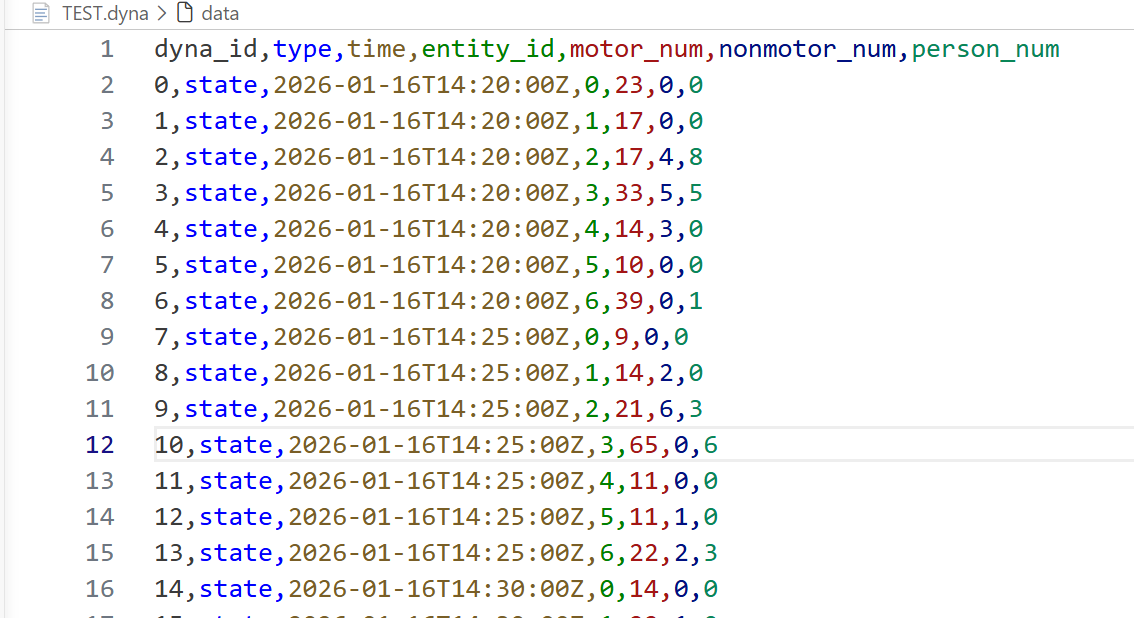
\includegraphics[width=0.9\textwidth]{figure/image3.png}
  \caption{处理后的流量数据（TEST.dyna）}
  \label{fig:dyna}
\end{figure}

\vspace{3em}